\begin{figure}[!ht]
    \centering
    \vspace{0.5cm}
    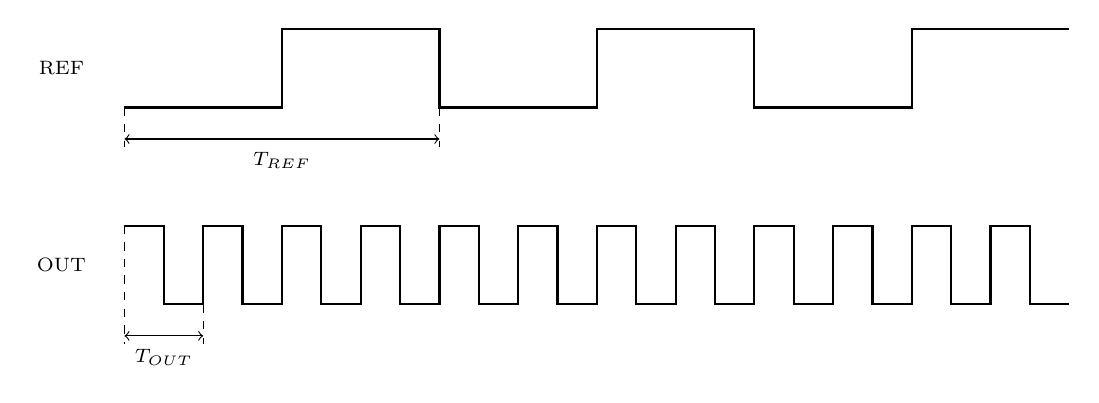
\begin{tikzpicture}

    \def \lref {0}
    \def \href {1}
    \def \lout {-2.5}
    \def \hout {-1.5}

    % Top signal: 3 periods of 4ns
    \draw[thick] (0,\lref) -- (2,\lref) -- (2,\href) -- (4,\href) -- (4,\lref) -- (6,\lref) -- (6,\href) -- (8,\href) -- (8,\lref) -- (10,\lref) -- (10,\href) -- (12,\href);
    \node at (-0.8,0.5) {\scriptsize REF};

    \draw (2,-0.45) node[anchor=north]{\scriptsize $T_\text{REF}$};
    \draw[<->] (0,-0.4) -- (4,-0.4);
    
    % Bottom signal: 12 periods of 1ns
    \draw[thick] (0,\hout) -- (0.5,\hout) -- (0.5,\lout) -- (1,\lout) -- (1,\hout) -- (1.5,\hout) -- (1.5,\lout) -- (2,\lout) -- (2,\hout) -- (2.5, \hout) -- (2.5,\lout) -- (3,\lout) -- (3,\hout) -- (3.5,\hout) -- (3.5,\lout) -- (4,\lout) -- (4,\hout) -- (4.5,\hout) -- (4.5,\lout) -- (5,\lout) -- (5,\hout) -- (5.5,\hout) -- (5.5,\lout) -- (6,\lout) -- (6,\hout) -- (6.5,\hout) -- (6.5,\lout) -- (7,\lout) -- (7,\hout) -- (7.5,\hout) -- (7.5,\lout) -- (8,\lout) -- (8,\hout) -- (8.5,\hout) -- (8.5,\lout) -- (9,\lout) -- (9,\hout) -- (9.5,\hout) -- (9.5,\lout) -- (10,\lout) -- (10,\hout) -- (10.5,\hout) -- (10.5,\lout) -- (11,\lout) -- (11,\hout) -- (11.5,\hout) -- (11.5,\lout) -- (12,\lout);
    \node at (-0.8,-2) {\scriptsize OUT};

    \draw (0.5,-2.95) node[anchor=north]{\scriptsize $T_\text{OUT}$};
    \draw[<->] (0,-2.9) -- (1,-2.9);

    \draw[dashed] (0,\lref) --++ (0,-0.5);
    \draw[dashed] (4,\lref) --++ (0,-0.5);
    \draw[dashed] (0,\hout) --++ (0,-1.5);
    \draw[dashed] (1,\lout) --++ (0,-0.5);
    
    \end{tikzpicture}
    \caption{Демонстрација рада синтетизатора учестаности за FMUL=4.}
    \label{fig:fll:fref_fout}
\end{figure}
